\documentclass{article}
\usepackage{hyperref}
\usepackage[margin=1in]{geometry}
\usepackage{indentfirst}
\usepackage{setspace} 
\usepackage{subdepth}
\usepackage{graphicx}
\graphicspath{{./images/}}
\doublespacing


\begin{document}
\title{Regular Languages and Finite State Machines}
\author{Remington Greko, Tyler Gutowski, Spencer Hirsch, Thomas Johnson}
\date{\today}

\maketitle

\begin{enumerate}
    \item \textbf{Read the \href{https://en.wikipedia.org/wiki/Regular_grammar}{Wikipedia} article on regular grammars. Summarize
            the saliet points.}

    \medskip

    \-\hspace{0.5cm} Briefly a regular grammar extends from a formal grammar. A formal grammar is given 
    by the definition of:
    \[G = (V, T, S, P)\]
    with
    
    \smallskip

    \-\hspace{0.5cm} \textit{V}: A finite set of \textbf{variables}. \\
    \-\hspace{0.5cm} \textit{T}: A finite set of \textbf{symbols}.  \\
    \-\hspace{0.5cm} \textit{S}: $S \in V$ being a \textbf{special} symbol called the \textbf{start symbol}.    \\
    \-\hspace{0.5cm} \textit{P}: Being a set of \textbf{productions}. 

    \-\hspace{0.5cm} With productions showing how symbols from \textit{V}, and \textit{S} may be used to create \textit{strings}.
    \[G = (\{S, A\}, \{a, b\}, S, P)\]
    \-\hspace{0.5cm} With productions being: \\
    \-\hspace{1.0cm} $S \Rightarrow ab$ \\
    \-\hspace{1.0cm} $S \Rightarrow aS$ \\
    \-\hspace{1.0cm} $S \Rightarrow bS$ \\
    \-\hspace{1.0cm} $S \Rightarrow \lambda$

    \-\hspace{0.5cm} Knowing this we can look at \textbf{regular grammars}

    \begin{itemize}
        \item \textbf{Strictly right-regular grammars}
    
        \medskip
        
        \-\hspace{0.5cm} These follow the production rule of $S \Rightarrow bA$ where 
        non terminal symbols from \textit{V} go on the right hand side 
        \item \textbf{Strictly left-regular grammars}
        
        \medskip

        \-\hspace{0.5cm} These follow the production rule of $S \Rightarrow Ab$ where 
        non terminal symbols from \textit{V} go on the left hand side 
        \item \textbf{Extended regular grammars}
        
        \medskip

        \-\hspace{0.5cm} These grammars will follow the production rules of either right, or left,
        $S \Rightarrow Ab $, where $b \in \sum^*$.
    \end{itemize}

    \medskip

    \item \textbf{What is a Deterministic Finite Accepter (DFA)?}
    
    \medskip

    % Answer here
    \-\hspace{0.5cm} A Deterministic Finite Accepter is a machine that can process an input
    string from left to right. A Finite Accepter is deterministic when there is only one thing
    that it can do for an input symbol. The DFA will either accept or reject the string. Once
    a String is accepted once, it will always be accepted. 

    \-\hspace{0.5cm} A DFA can only read left to right, just as traditional in the English
    language. The DFA can only see one specific element of a string at a time, it cannot go 
    backwards, nor skip ahead. A DFA also has a specific number of internal states, each
    different based on its current situation, such as when beginning a string. 

    \-\hspace{0.5cm} The example from the book is a great example of a Deterministic Finite Accepter,
    
    \[M = (Q, \Sigma, \delta, q_0, F)\]

    where

    \smallskip

    \-\hspace{0.5cm} \textit{Q} is a finite set of \textbf{internal states}, \\
    \-\hspace{0.5cm} $\Sigma$ is a finite set of symbols called the \textbf{input alphabet}, \\
    \-\hspace{0.5cm} $\delta$: \textit{Q} $\times$ $\Sigma$ $\rightarrow$ \textit{Q} is a total function called the 
    \textbf{transition function}, \\
    \-\hspace{0.5cm} \textit{$q_0$ $\in$ Q} is the \textbf{initial state}, \\
    \-\hspace{0.5cm} \textit{F \ $\subseteq$ Q} is a set of \textbf{final states}.



    \medskip

    \item \textbf{What is a Non-Deterministic Finite Accepter (NFA)?}
    
    \medskip

    \-\hspace{0.5cm} A non-deterministic finite acceptor can also be defined with the same formal definition
    of a deterministic finite accepter.
    \[M = (Q, \Sigma, \delta, q_0, F)\]

    \-\hspace{0.5cm} However an NFA has three main differences from a DFA.

    \begin{itemize}
        \item The range of $\delta$ is a subset of \textit{Q}. Meaning the range is $2^\delta$
        \item $\lambda$ is allowed as input for the transition function $\delta(q_1, \lambda)$
        \item The transfer function may equal an empty set. $\delta(q_i, a) = {\emptyset}$
    \end{itemize}

    \-\hspace{0.5cm} A brief encapsulation of the above topics is that an NFA has the power of choice. Given 
    an input character the transition function has multiple internal states to choose from. A NFA has clear advantages over a DFA for its more practical
    applications. Most complex problems can't always be solved deterministically without performing exhaustive
    backtracking based searches due to their linear design. This makes a NFA ideal for simulation
    of search-backtracking



    \medskip

    \item \textbf{Explain why the languages accepted by DFAs and NFAs are the equivalent.}
    
    \medskip

    % Answer here
    \-\hspace{0.5cm} Any language accepted by a DFA can also be accepted by an NFA,
     and vice versa. We can prove this through the use of the "subset construction
     algorithm." The core principle of this algorithm is the DFA simulates the NFA
     by keeping track of the every possible state. Each state of the DFA corresponds
     to a subset of the sets of the NFA.

     \-\hspace{0.5cm} As long as the languages are equivalent then both a DFA and an 
     NFA can be used when using the language. Although a DFA can only consist of a 
     fixed number of processes, those processes are a subset of the NFA processes,
     therefore languages accepted by both the DFA and the NFA are equivalent.

    \medskip

    \item \textbf{Give a recursive definition of \textit{regular expression} over
            an alaphabet $\Sigma$.}

    \medskip

    \-\hspace{0.5cm} A regular expression can be constucted by repeatedly applying
    recursive rules to primitive constituents. The algorithmic process is defined 
    below.

    \-\hspace{0.5cm} Let $\Sigma$ be a given alphabet. Apply the following steps:

    \begin{enumerate}
        \item $\emptyset$, $\lambda$, and $\alpha$ $\in$ $\Sigma$ are all regular
        expressions. All of these are \textbf{primitive regular expressions}.
        \item If \textit{r}\textsubscript{1} and \textit{r}\textsubscript{2} are
        regular expressions, so are \textit{r}\textsubscript{1} + 
        \textit{r}\textsubscript{2}, $\textit{r}\textsubscript{1} \cdot
        \textit{r}\textsubscript{2}$, $r_1^*$, and (\textit{r}\textsubscript{1}).
        \item A string is a regular expression iff it can be derived from the 
        primitive regular expressions by a finite number of applications of the
        rules in step (b).
    \end{enumerate}


    \medskip

    \item \textbf{Confirm you know how to use operating system commands to find
            regular expressions in a file.}	\\
	\medskip
	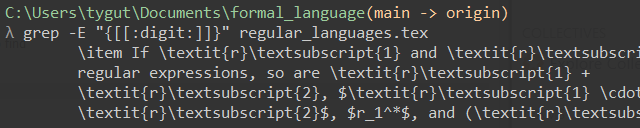
\includegraphics{regex_proof} \\
	The operating system command used, \textbf{grep -E "$\{$[[:digit:]]$\}$" regular\_languages.tex} uses \textbf{grep} (global regular expression print) with the parameter \textbf{-E}, which is shorthand for \textbf{--regex-extended}. The regex phrase \textbf{"$\{$[[:digit:]]$\}$"} is then searched, which is any numeral inside of curly braces. As shown on the four lines below the command, there were several instances of a numeral within curly braces, all of which were a part of \textbf{textsubscript$\{$$\}$}. \\


    \medskip

    % Answer here

    \medskip
\end{enumerate}

\pagebreak

\begin{center}
    \begin{tabular}{|p{3cm}|p{6cm}|}
        \hline
        \textbf{Name} & \textbf{Section} \\
        \hline
        Remington Greko &  Question 5\\
        \hline
        Tyler Gutowski &  Question 6\\
        \hline
        Spencer Hirsch &  Question 2 and 4\\
        \hline
        Thomas Johnson &  Question 1 and 3\\
        \hline
    \end{tabular}
\end{center}

\end{document}
